\TieudeT{PHONG TỎA VẬT LÍ 12 - VẬT LÍ NHIỆT}
\subsubsection*{PHẦN I. Thí sinh trả lời câu hỏi từ câu 1 đến câu 18. Mỗi câu hỏi thí sinh chỉ chọn một phương án}
\setcounter{ex}{0}
\begin{ex}%group
	\immini[thm]{Cho sơ đồ quá trình chuyển thể như hình bên. Phát biểu nào sau đây là đúng?
		\choice
		{$(3)$ là quá trình ngưng tụ}
		{\True $(2)$ là quá trình thăng hoa}
		{$(1)$ là quá trình nóng chảy}
		{$(4)$ là quá trình thăng hoa}}
	{	\begin{tikzpicture}[line cap=butt,line join=miter,>=stealth,scale=0.5]
			
			%		\draw[red,->,line width =3] (-3,0)-- (1,0) (-3,0.3) -- (0,4.3) (-3,-0.3) -- (0,3.7) ;
			\draw[red,->,line width =1] (-3,0)-- (2,0) node[below, midway]{(2)};
			\draw[red,->,line width=1] (3,0) -- ({0 +3/5}, {4 - 4/5})node[below,left, midway]{(4)};
			\draw[red,->,line width =1,xshift=-8,yshift=10] (-3,0) -- (0-3/5,4-4/5) node[above,left, midway]{(3)} ;
			\draw[red,->,line width =1, xshift=8, yshift=-8]  (0,4) --(-3+3/5,0+4/5) node[below,yshift=-3, midway]{(1)};
			
			
			\path[draw=red, fill=white] (-3,0) circle (1) node {rắn} (3,0) circle (1) node {khí} (0,4) circle (1) node {lỏng} ;
			
	\end{tikzpicture}}
	%	{\includegraphics[width=0.3\linewidth]{Images/920142}}
	\loigiai{
		Quá trình (2) là quá trình thăng hoa.
	}
\end{ex}
\begin{ex}%group
	Với cùng một chất, quá trình chuyển thể nào sẽ làm giảm lực tương tác giữa các phân tử nhiều nhất?
	\choice 
	{Ngưng tụ}
	{Đông đặc}
	{\True Hóa hơi}
	{Nóng chảy}
	\loigiai{
		\begin{itemize}
			\item Với cùng một chất, quá trình chuyển thể sẽ làm giảm lực tương tác giữa các phân tử nhiều nhất là hóa hơi.
		\end{itemize}
	}
\end{ex}
\begin{ex}%group
	Hệ thức định luật I nhiệt động lực học $\Delta U=A+Q$. Khi $Q<0$ và $A>0$ mô tả quá trình 
	\choice
	{vật dẫn nhiệt và sinh công}
	{vật truyền nhiệt và sinh công}
	{vật dẫn nhiệt và nhận công}
	{\True vật truyền nhiệt và nhận công}
	\loigiai{\begin{itemize}
			\item Hệ thức định luật I nhiệt động lực học khi $Q<0$ và $A>0$ mô tả quá trình vật truyền nhiệt và nhận công.
			
	\end{itemize}}
\end{ex}
\begin{ex}%group
	Phát biểu nào sau đây là đúng?
	\choice
	{\True Vật làm bằng chất có nhiệt dung riêng nhỏ thì vật đó dễ nóng lên và nhanh nguội đi}
	{Vật làm bằng chất có nhiệt dung riêng nhỏ thì vật đó dễ nóng lên và lâu nguội đi}
	{Vật làm bằng chất có nhiệt dung riêng nhỏ thì vật đó khó nóng lên và nhanh nguội đi}
	{Vật làm bằng chất có nhiệt dung riêng nhỏ thì vật đó khó nóng lên và lâu nguội đi}
	\loigiai{
		Vật làm bằng chất có nhiệt dung riêng nhỏ thì vật đó dễ nóng lên và nhanh nguội đi.
	}
\end{ex}
\begin{ex}%group
	Hình bên là dự báo thời tiết ở thành phố Hồ Chí Minh ngày $21/07/2024$. Theo thang nhiệt Kelvin, nhiệt độ cao nhất và thấp nhất theo bảng dự báo bên là
	\begin{center}
		\begin{tikzpicture}
			%\draw [dotted] (-2,-2) grid (14,4);
			%Hình 1
			\draw [rounded corners](-1.2,-1.5) rectangle (1.2,2);
			\node [star, star points=12, star point ratio=0.4, draw, fill=yellow, minimum size=1cm, scale=0.5] at (0.4,0.4) {};
			\begin{scope}[shift={(0.5,-0.5)}]
				\draw [fill = yellow, rotate=-20] (0,0.5) -- (-0.2,-0.2) -- (-0.1,-0.2) -- (-0.2,-0.2-0.7) -- (0,-0.1)--(-0.1,-0.1)--cycle ;
			\end{scope}
			\node[cloud, draw, minimum width=2cm, minimum height=1cm, fill=blue!50] at (0,0) {};
			\foreach \x/\y in {-0.5/-0.5,-0.2/-0.9,0.1/-0.7,0.
				4/-0.8,0.7/-0.4,0.9/-0.7}{
				\draw [fill = blue, rotate=-20] (\x,\y) .. controls (\x-0.2,\y-0.2) and (\x+0.2,\y-0.2) .. (\x,\y);
			}
			\draw 
			node[above] at (0,1) {$28^\circ C$}
			node[above] at (0,1.5) {10:00};
			%Hình 2
			\begin{scope}[shift={(3,0)}]
				\draw [rounded corners](-1.2,-1.5) rectangle (1.2,2);
				\node [star, star points=12, star point ratio=0.4, draw, fill=yellow, minimum size=1cm, scale=0.5] at (0.4,0.4) {};
				\begin{scope}[shift={(0.5,-0.5)}]
					\draw [fill = yellow, rotate=-20] (0,0.5) -- (-0.2,-0.2) -- (-0.1,-0.2) -- (-0.2,-0.2-0.7) -- (0,-0.1)--(-0.1,-0.1)--cycle ;
				\end{scope}
				\node[cloud, draw, minimum width=2cm, minimum height=1cm, fill=blue!50] at (0,0) {};
				\foreach \x/\y in {-0.5/-0.5,-0.2/-0.9,0.1/-0.7,0.
					4/-0.8,0.7/-0.4,0.9/-0.7}{
					\draw [fill = blue, rotate=-20] (\x,\y) .. controls (\x-0.2,\y-0.2) and (\x+0.2,\y-0.2) .. (\x,\y);
				}
				\draw 
				node[above] at (0,1) {$32^\circ C$}
				node[above] at (0,1.5) {13:00};
			\end{scope}
			%Hình 3
			\begin{scope}[shift={(6,0)}]
				\draw [rounded corners](-1.2,-1.5) rectangle (1.2,2);
				\node [star, star points=12, star point ratio=0.4, draw, fill=yellow, minimum size=1cm, scale=0.5] at (0.4,0.4) {};
				\begin{scope}[shift={(0.5,-0.5)}]
					\draw [fill = yellow, rotate=-20] (0,0.5) -- (-0.2,-0.2) -- (-0.1,-0.2) -- (-0.2,-0.2-0.7) -- (0,-0.1)--(-0.1,-0.1)--cycle ;
				\end{scope}
				\node[cloud, draw, minimum width=2cm, minimum height=1cm, fill=blue!50] at (0,0) {};
				\foreach \x/\y in {-0.5/-0.5,-0.2/-0.9,0.1/-0.7,0.
					4/-0.8,0.7/-0.4,0.9/-0.7}{
					\draw [fill = blue, rotate=-20] (\x,\y) .. controls (\x-0.2,\y-0.2) and (\x+0.2,\y-0.2) .. (\x,\y);
				}
				\draw 
				node[above] at (0,1) {$30^\circ C$}
				node[above] at (0,1.5) {15:00};
			\end{scope}
			%Hình 4
			\begin{scope}[shift={(9,0)}]
				\draw [rounded corners](-1.2,-1.5) rectangle (1.2,2);
				\node [star, star points=12, star point ratio=0.4, draw, fill=yellow, minimum size=1cm, scale=0.5] at (0.4,0.4) {};
				\begin{scope}[shift={(0.5,-0.5)}]
					\draw [fill = yellow, rotate=-20] (0,0.5) -- (-0.2,-0.2) -- (-0.1,-0.2) -- (-0.2,-0.2-0.7) -- (0,-0.1)--(-0.1,-0.1)--cycle ;
				\end{scope}
				\node[cloud, draw, minimum width=2cm, minimum height=1cm, fill=blue!50] at (0,0) {};
				\foreach \x/\y in {-0.5/-0.5,-0.2/-0.9,0.1/-0.7,0.
					4/-0.8,0.7/-0.4,0.9/-0.7}{
					\draw [fill = blue, rotate=-20] (\x,\y) .. controls (\x-0.2,\y-0.2) and (\x+0.2,\y-0.2) .. (\x,\y);
				}
				\draw 
				node[above] at (0,1) {$27^\circ C$}
				node[above] at (0,1.5) {15:00};
			\end{scope}
			\draw
			node[above] at (4.5,2) {Tp Hồ Chí Minh, ngày 21/07/2024};
		\end{tikzpicture}
	\end{center}
	\choice 
	{$246\ K$ và $241\ K$}
	{\True $305\ K$ và $300\ K$}
	{$248\ K$ và $236\ K$}
	{$321\ K$ và $306\ K$}
	\loigiai{
		Dựa vào hình, ta thấy:
		$\begin{cases}
			t_{max} = 32^\circ C &\Rightarrow T_{max} = 305\ K\\
			t_{min} = 27^\circ C &\Rightarrow T_{min} = 300\ K
		\end{cases}$.
	}
\end{ex}
\begin{ex}%group
	\immini[thm]{
		Hai chất rắn $A$ và $B$ được làm nóng chảy trong cùng một lò nung. Đồ thị sự phụ thuộc của nhiệt độ vào thời gian của $A$ và $B$ được biểu diễn như hình vẽ. Nếu $A$ và $B$ có cùng khối lượng, phát biểu nào sau đây là đúng?}{
		\begin{tikzpicture}[scale = 1, line join=round, line cap=round, >=stealth,line width=1.5]
			\draw[->] (0,0) node [below] {O} -- (0,4) node [left] {Nhiệt độ};
			\draw[->] (0,0) -- (4,0) node [below] {Thời gian};
			\draw[red] (0,1.5) -- (1,2.5) -- (3,2.5) -- (3.5,3) node [right] {B};
			\draw[blue] (0,1.5) -- (1,3) -- (2.7,3) -- (3.1,3.5) node [right] {A};
			\draw[line width=0.5,dashed] (1,3) -- (1,0);
	\end{tikzpicture}}
	\choice
	{\True Chất rắn $A$ có nhiệt nóng chảy riêng và nhiệt dung riêng nhỏ hơn chất rắn $B$}
	{Chất rắn $A$ có nhiệt nóng chảy riêng và nhiệt dung riêng lớn hơn chất rắn $B$}
	{Chất rắn $A$ có nhiệt nóng chảy riêng lớn hơn B nhưng nhiệt dung riêng nhỏ hơn $B$}
	{Chất rắn $A$ có nhiệt nóng chảy riêng nhỏ hơn B nhưng nhiệt dung riêng lớn hơn $B$}
	\loigiai{
		Từ đồ thị ta thấy thời gian nóng chảy của $B$ lớn hơn thời gian nóng chảy của $A$ nên nhiệt lượng cần cung cấp cho $B$ nóng chảy lớn hơn $A$ Do khối lượng của $2$ chất bằng nhau nên $B$ có nhiệt nóng chảy riêng lớn hơn $A$.\\
		Từ đồ thị ta cũng thấy, trong cùng $1$ khoảng thời gian nhận nhiệt nhưng nhiệt độ của $A$ lớn hơn của $B$ nên nhiệt dung riêng của $A$ nhỏ hơn nhiệt dung riêng của $B$\\
		Vậy $A$ có nhiệt nóng chảy riêng và nhiệt dung riêng nhỏ hơn $B$ 
	}
\end{ex}
\begin{ex}%group
	Rạng sáng ngày $1/12/2014$ một đường ống dẫn nước tưới cây của thành phố Bắc Kinh (Trung Quốc) bị vỡ đã tạo khung cảnh băng tuyết tráng lệ khiến cư dân thành phố này thích thú và háo hức đi xem. Sự cố xảy ra hiện tượng vỡ đường ống nước là do
	\choice
	{trời lạnh làm đường ống bị cứng giòn và rạn nứt}
	{tuyết rơi nhiều đè nặng lên thành ống}
	{sự chênh lệch nhiệt độ bên trong và bên ngoài ống làm ống nứt vỡ}
	{\True thể tích nước khi đông đặc tăng lên gây ra áp lực lớn lên thành ống}
	\loigiai{
		Sự cố xảy ra hiện tượng vỡ đường ống nước là do thể tích nước khi đông đặc tăng lên gây ra áp lực lớn lên thành ống.
	}
\end{ex}
\begin{ex}%group
	\immini[thm]{Hơ nóng một khối khí trong ống nghiệm có nút đậy kín (không quá chặt) như hình $a$ và kết quả nút bật ra khỏi ống nghiệm (hình $b$). Phát biểu nào sau đây là \textbf{sai}?}{\definecolor{cc5584e}{RGB}{197,88,78}
		
		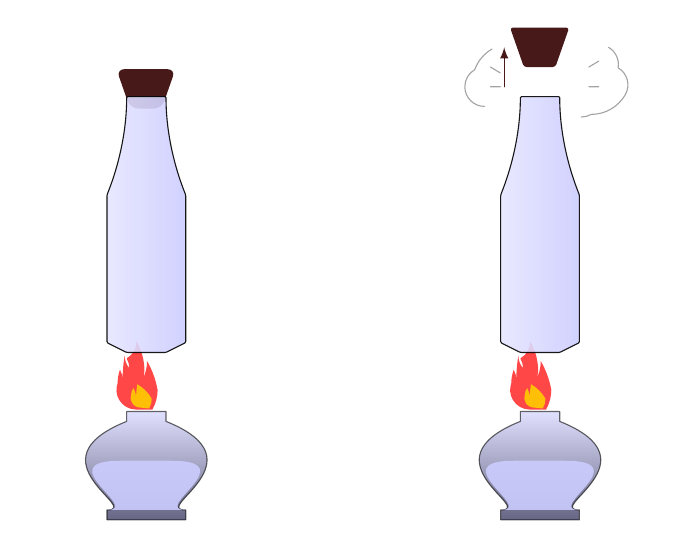
\begin{tikzpicture}[line cap=round,line join=round,scale=0.5]
			%nhiệt kế
			\begin{scope}[shift={(0,0)}]
				
				% bình cồn
				\path[draw =black,top color=blue!20!white,bottom color=blue!20!black,opacity=0.6] (-4.62,-4.95)-- (-4.62,-4.7)
				..controls(-3.73,-4.7)and(-6.62,-3.45)
				..
				(-4.12,-2.45)-- (-4.12,-2.2) -- (-3.12,-2.2) -- (-3.12,-2.45)
				..controls(-0.62,-3.45)and(-3.52,-4.7)
				..
				(-2.62,-4.7)-- (-2.62,-4.95)--cycle;
				\path[fill=blue!20,opacity=0.9] (-4.62,-4.7)
				..controls(-3.73,-4.7)and(-6.12,-3.45)
				..
				(-4.28,-3.45)-- (-2.98,-3.45)
				..controls(-1.12,-3.45)and(-3.52,-4.7)
				..
				(-2.62,-4.7)--cycle;
				
				%lữa
				\path[fill=red!80,opacity=0.9](-3.88,-2.15)arc(-90:-200:0.5)arc(-180:-200:1)arc(30:0:0.5)arc(180:170:3.5)arc(180:220:0.5)arc(0:30:0.5)arc(-60:0:0.5)arc(30:0:1.5)arc(0:-30:0.5)arc(-30:0:1)arc(30:10:2.25)arc(0:-30:1)--cycle;
				\path[fill=red!20!yellow,opacity=0.9,line width=0.5](-3.77,-2.1)arc(-90:-200:0.25)arc(-180:-220:0.25)arc(30:0:0.5)arc(180:170:2)arc(60:30:1)arc(0:-30:0.5)--cycle;
				
				%nắp chai
				\path[opacity=0.9,fill=red!20!black,rounded corners=0.1cm,yshift=-30] (-4.03,6.55)-- (-3.23,6.55) --
				(-2.88,7.55)
				-- (-4.38,7.55) --cycle;
				
				
				
				
				
				\path[draw=black,left color=blue!10!white,right color=blue!20,,opacity=0.9,rounded corners=0.4] (-3.12,5.8)
				..controls(-3.12,5.55)and(-3.12,4.55)
				..
				(-2.62,3.3)
				-- (-2.62,-0.45) -- (-3.12,-0.7) -- (-4.12,-0.7) -- (-4.62,-0.45) -- (-4.62,3.3)
				..controls(-4.12,4.55)and(-4.12,5.55)
				..
				(-4.12,5.8) --cycle;
				
				% Image image1 not included. Base64 still not supported		;
			\end{scope}
			%----------------------
			\begin{scope}[shift={(10,0)}]
				
				% bình cồn
				\path[draw =black,top color=blue!20!white,bottom color=blue!20!black,opacity=0.6] (-4.62,-4.95)-- (-4.62,-4.7)
				..controls(-3.73,-4.7)and(-6.62,-3.45)
				..
				(-4.12,-2.45)-- (-4.12,-2.2) -- (-3.12,-2.2) -- (-3.12,-2.45)
				..controls(-0.62,-3.45)and(-3.52,-4.7)
				..
				(-2.62,-4.7)-- (-2.62,-4.95)--cycle;
				\path[fill=blue!20,opacity=0.9] (-4.62,-4.7)
				..controls(-3.73,-4.7)and(-6.12,-3.45)
				..
				(-4.28,-3.45)-- (-2.98,-3.45)
				..controls(-1.12,-3.45)and(-3.52,-4.7)
				..
				(-2.62,-4.7)--cycle;
				
				%lữa
				\path[fill=red!80,opacity=0.9](-3.88,-2.15)arc(-90:-200:0.5)arc(-180:-200:1)arc(30:0:0.5)arc(180:170:3.5)arc(180:220:0.5)arc(0:30:0.5)arc(-60:0:0.5)arc(30:0:1.5)arc(0:-30:0.5)arc(-30:0:1)arc(30:10:2.25)arc(0:-30:1)--cycle;
				\path[fill=red!20!yellow,opacity=0.9,line width=0.5mm](-3.77,-2.1)arc(-90:-200:0.25)arc(-180:-220:0.25)arc(30:0:0.5)arc(180:170:2)arc(60:30:1)arc(0:-30:0.5)--cycle;
				
				%nắp chai
				\path[opacity=0.9,fill=red!20!black,rounded corners=1] (-4.03,6.55)-- (-3.23,6.55) --
				(-2.88,7.55)
				-- (-4.38,7.55) --cycle;
				
				\path[opacity=0.9,draw=red!20!black,rounded corners=0.1,-latex] (-4.53,6.05)--
				++(0,1);
				
				\path[draw=gray!80,opacity=0.9](-5.03,5.55)arc(-90:-240:0.5)arc(-200:-240:1) (-1.88,7.05)arc(60:-10:0.5)arc(60:-30:0.5)arc(-30:-90:1)arc(-60:-90:0.5) (-2.38,6.55)-- ++(0.25,0.15) (-2.38,6.05)-- ++(0.25,0) (-4.88,6.05)-- ++(0.25,0) (-4.88,6.55)--
				++(0.25,-0.15);
				
				\path[draw=black,left color=blue!10!white,right color=blue!20,,opacity=0.9,rounded corners=0.4] (-3.12,5.8)
				..controls(-3.12,5.55)and(-3.12,4.55)
				..
				(-2.62,3.3)
				-- (-2.62,-0.45) -- (-3.12,-0.7) -- (-4.12,-0.7) -- (-4.62,-0.45) -- (-4.62,3.3)
				..controls(-4.12,4.55)and(-4.12,5.55)
				..
				(-4.12,5.8) --cycle;
				
				% Image image1 not included. Base64 still not supported		;
			\end{scope}
	\end{tikzpicture}}
	
	%{\includegraphics[width=6 cm]{images/LeMinhAnh-De31-THTNguyenKhuyen-2}}
	\choice
	{Khi bị đốt nóng, nội năng của khí trong ống nghiệm tăng lên}
	{Áp suất khí trong ống tăng lên tạo ra lực đẩy đủ lớn làm bật nút đẩy ra khỏi ống nghiệm}
	{\True Nội năng của khí trong ống nghiệm tăng là do thế năng của các phân tử khí tăng còn động năng phân tử khí không tăng}
	{Khi nhiệt độ tăng thì các phân tử khí va chạm với thành bình nhiều và mạnh hơn}
	\loigiai{
		\begin{itemize}
			\item Nhiệt độ tăng thì động năng phân tử khí tăng, thế năng tương tác giữa phân tử khí không đáng kể.
		\end{itemize}
	}
\end{ex}
\begin{ex}%group
	\immini[thm]
	{Hình bên là đường biểu diễn sự thay đổi nhiệt độ theo thời gian khi làm lạnh nước tinh khiết. Phát biểu nào dưới đây là đúng?
		\choice 
		{\True Từ phút thứ năm đến phút thứ sáu, nước ở cả thể lỏng và thể rắn}
		{Từ phút thứ nhất đến phút thứ hai, nước ở thể rắn}
		{Từ phút thứ hai đến phút thứ mười, nhiệt độ của nước không đổi}
		{Nhiệt độ của nước giảm đều theo thời gian}}
	{\begin{tikzpicture}[>=stealth, thick]
			%\draw[dotted] (-2,-2) grid (7,5);
			\draw [->] (0,-1) -- (0,4.5);
			\draw [->] (0,0) -- (7,0);
			\foreach \x in {1,...,6}{
				\draw
				(\x,0.1) -- (\x,-0.1)
				(0.1,\x-2) -- (-0.1,\x-2);
			}
			\draw 
			node [left] at (0,0) {$O$}
			node [left] at (0,2) {$5$}
			node [left] at (0,4) {$10$}
			node [below] at (3,0) {$5$}
			node [below] at (6,0) {$10$}
			node [right] at (0,4.5) {Nhiệt độ $\left(^\circ C\right)$}
			node [above] at (7,0) {Thời gian(phút)};
			\draw (0,4).. controls (0.5,2) and (1,1) .. (2,0) -- (5,0) [out = -10, in = 100] to (6,-1);
	\end{tikzpicture}}
	\loigiai{
		Dựa vào đồ thị, ta thấy $\dfrac{10}{3} \leq t \leq \dfrac{25}{3}$ (phút) nước trong quá trình đông đặc 
	}
\end{ex}
%Câu 13

%Câu 14
\begin{ex}%group
	Một viên đạn đại bác có khối lượng $10\ kg$ khi rơi tới đích có vận tốc $54\ km/h$. Nếu toàn bộ động năng của nó biến thành nội năng thì nhiệt lượng tỏa ra lúc va chạm vào khoảng
	\choice 
	{$14580\ J$}
	{$2250\ J$}
	{\True $1125\ J$}
	{$7290\ J$}
	\loigiai{
		Theo đề bài, ta có: $Q = W_\text{đ} = \dfrac{1}{2}mv^2 = \dfrac{1}{2}10.15^2 =1125\ J$.
	}
\end{ex}

\begin{ex}%group%group
	Bỏ $100\ g$ nước đá ở $t_1=0^\circ C$ vào $300\ g$ nước ở $t_2=20^\circ C$. Cho nhiệt nóng chảy riêng của nước đá là $\lambda =3,4.10^5\ J/kg$ và nhiệt dung riêng của nước là $c = 4200\ J/kg.K$. Bỏ qua sự hao phí nhiệt ra môi trường. Khi xảy ra cân bằng nhiệt, khối lượng nước đá còn lại là 
	\choice
	{$16\ g$}
	{$20\ g$}
	{\True $26\ g$}
	{$62\ g$}
	\loigiai{
		\begin{itemize}
			\item 	Nhiệt lượng cần cung cấp cho 100 g nước đá để nó tan hoàn toàn là 
			$$ Q_1 = m_1\lambda  = 0,1.3,4.10^5 = 34000 \ J.$$
			\item 	Nhiệt lượng tỏa ra của $300\ g$ nước khi hạ nhiệt độ từ $20^\circ C$ xuống $0^\circ C$  là 
			$$Q_2 = m_2c\Delta t = 0,3.4200.(20-0) = 25200 \ J.$$
			\item 	Vì $Q_1 > Q_2$ nên nước đá không tan hoàn toàn, ta có 
			$$Q_2 = m’\lambda\Rightarrow m’ = 74 g\Rightarrow \Delta m = m_1 - m' = 26\ g$$
			
		\end{itemize}
	}
\end{ex}

\begin{ex}%group
	Hình bên biểu diễn sự thay đổi nhiệt độ theo thời gian của nước khi được đun nóng và để nguội. Thời gian nước sôi là
		\begin{center}
			\begin{tikzpicture}[scale=0.4, >=stealth, font=\footnotesize, line join=round, line cap=round]
				\draw[->] (0,0) -- (22,0) node[above right] {Thời gian (phút)};
				\draw[->] (0,0) -- (0,12) node[above] {Nhiệt độ ($^\circ C$)};
				\coordinate (A) at (0,0);
				\coordinate (B) at (10,10);
				\coordinate (C) at (14,10);
				\coordinate (D) at (20,2);
				\draw[thick] (A) -- (B) node[above]{$\large{B}$} -- (C)node[above]{$\large{C}$} -- (D)node[right]{$\large{D}$};
				%		\foreach \point/\label/\position in {B/B/above, C/C/above, D/D/right}{\node[\position] at (\point) {\label};}
				\foreach \x in {2,4,...,20}
				\draw[dashed, gray!80] (\x,0) -- (\x,10);
				\foreach \y in {2,4,6,8,10}
				\draw[dashed, gray!80] (0,\y) -- (20,\y);
				\foreach \x/\xlabel in {0/0, 10/10, 20/20}
				\node[below] at (\x,0) {\xlabel};
				\foreach \y/\ylabel in {2/20, 4/40, 6/60, 8/80, 10/100}
				\node[left] at (0,\y) {\ylabel};
			\end{tikzpicture}
		\end{center}
		\choice
		{8 phút}
		{6 phút}
		{2 phút}
		{\True 4 phút}
	 	
	
	\loigiai{
		\begin{itemize}
			\item Từ hình bên, ta thấy thời gian nước sôi là $14-10=4\ \text{(phút)}$.
		\end{itemize}
	}
\end{ex}
\begin{ex}%group
	Độ Fahrenheit là một thang nhiệt độ được đặt theo tên nhà vật lý người Đức Daniel Gabriel Fahrenheita), ngày nay vẫn được sử dụng rộng rãi ở Mỹ và một số quốc gia nói tiếng Anh. Công thức chuyển đổi giữa thang nhiệt độ Fahrenheit và thang nhiệt độ Celcius là $t(^\circ F)=32+1,8t(^\circ C)$. Nhiệt dung riêng của nước ứng với thang nhiệt độ Celsius là $4200\ J/kg.^\circ C$. Trong thang nhiệt độ Fahrenheit, nhiệt dung riêng của nước có giá trị xấp xỉ
	\choice
	{$7560\ J/kg.^\circ F$}
	{\True $2333,3\ J/kg.^\circ F$}
	{$124,3\ J/kg.^\circ F$}
	{$131,2\ J/kg.^\circ F$}
	\loigiai{
		\begin{itemize}
			\item Ta có: $Q=mc.\Delta t \Rightarrow c=\dfrac{Q}{m \Delta t}\ (\dfrac{J}{kg.K})$
			\item Mà độ biến thiên nhiệt độ theo thang Kevin bằng độ biến thiên nhiệt độ theo thang Celcius.
			\item Và $t(^\circ F)=32+1,8t(^\circ C) \Rightarrow \Delta t(^\circ F)=1,8\Delta t(^\circ C)$
			\item Suy ra $c=4200\ (\dfrac{J}{kg.^\circ C})=\dfrac{4200}{1,8}\ (\dfrac{J}{kg.^\circ F}) \approx 2333,3\ (\dfrac{J}{kg.^\circ F})$.
		\end{itemize}
	}
\end{ex}
\begin{ex}%group
	\immini[thm]
	{
		Cung cấp năng lượng nhiệt cho một vật, công suất phụ thuộc theo thời gian được biểu diễn như hình vẽ. Thời điểm vật nhận được nhiệt lượng $40\ J$ tính từ thời điểm ban đầu là
		\choice
		{$6\ s$}
		{$5\ s$}
		{\True $4\ s$}
		{$3\ s$}   
	}
	{
		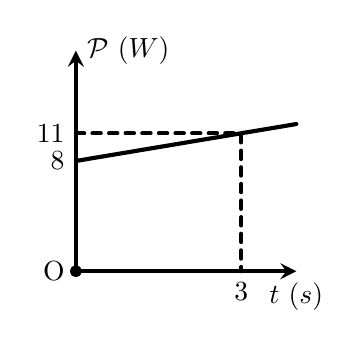
\begin{tikzpicture}[scale = 0.7, line join=round, line cap=round, >=stealth,line width=1.5]
			\draw[->,line width=1.5] (0,0) -- (4,0) node[below] {$t\  (s)$};
			\draw[->,line width=1.5] (0,0) -- (0,4) node[right] {$\mathcal{P}\ (W)$};
			\draw[fill = black] (0,0) node [left] {O} circle(2pt);
			\draw[-,thick, line width = 1.5] (0,2)node[left]{8} -- (4,2.67) ;
			\draw[dashed] (0,2.5)node[left]{11}--(3,2.5)--(3,0)node[below]{3};
			
		\end{tikzpicture}  
	}
	\loigiai{
		$\mathcal{P}=at+b \Rightarrow
		\begin{cases}
			8 = a.0+b\\
			11=a.3+b
		\end{cases}
		\Rightarrow
		\begin{cases}
			a=1\\
			b=8
		\end{cases} 
		\rightarrow \mathcal{P}=t+8$\\
		$Q=\overline{\mathcal{P}}t=\dfrac{(0+8)+(t+8)}{2}t=\dfrac{1}{2}t^2+8t=40\Rightarrow t=4\ s$
	}
\end{ex}
\begin{ex}%group
	Người khỏe mạnh có thân nhiệt trung bình là $37^\circ C$. Theo độ Kelvin thì nhiệt độ thân nhiệt trung bình của người khỏe mạnh là
	\choice
	{\True $310\ K$}
	{$37\ K$}
	{$236\ K$}
	{$273\ K$}
	\loigiai{
		$T(K) = t(^\circ C)+273 = 37+273=310\ K$
	}
\end{ex}
\begin{ex}%group
	Laser (Laze) được sử dụng để khoan kim loại vì nó có thể tạo ra một chùm tia sáng với năng lượng lớn, tập trung vào một điểm nhỏ và có độ chính xác cao. Dùng một mũi khoan laser có công suất $200\ W$ để khoan vào một khối kim loại. Biết nhiệt nóng chảy riêng của kim loại là $250\ J/g$, khối lượng riêng của kim loại là $7,8\  {g/cm}^{3}$ và đường kính mũi khoan là $0,2\ cm$. Giả sử đã nung nóng kim loại đến nhiệt độ nóng chảy để khoan. Lấy $\pi = 3,14$. Thời gian tối thiểu để khoan qua một lỗ tròn có độ dày $0,5\ cm$ là
	\choice
	{$0,252\ s$}
	{$0,604\ s$}
	{$0,323\ s$}
	{\True $0,153\ s$}
	\loigiai{
		\begin{itemize}
			\item Thể tích phần kim loại cần làm nóng chảy là: $V = S.h = \pi r^2.h = 3,14.(0,1)^2.0,5=15,7.10^{-3}\ cm^3$
			\item Khối lượng phần kim loại cần làm nóng chảy là: $m=V.\rho = 15,7.10^{-3}.7,8 = 122,46.10^{-3}\ (g)$
			\item Nhiệt lượng cần để làm nóng chảy phần kim loại là:  $Q=m.\lambda ={{122,46.10}^{-3}}.250=30,615\,\,\left( J \right)$.
			\item Thời gian tối thiểu để khoan qua một lỗ tròn có độ dày 0,5 cm là: $t=\frac{Q}{P}=\frac{30,615}{200}\approx 0,153\,\,\left( s \right)$.
		\end{itemize}
	}
\end{ex}
\begin{ex}%group
	Khi thực hành trong phòng thí nghiệm, một học sinh cho một luồng hơi nước ở $100^\circ C$ ngưng tụ trong một nhiệt lượng kế chứa $0,55\ kg$ nước ở $20^\circ C$, kết quả là nhiệt độ của nước tăng lên đạt nhiệt độ cân bằng là $47,3^\circ C$ và khối lượng nước trong nhiệt kế tăng thêm $0,03\ kg$. Biết nhiệt dung riêng của nước bằng $4200\ J/kg.K$. Nhiệt hoá hơi riêng của nước có giá trị bằng
	\choice
	{$1,28.10^6\ J/kg$}
	{$1,38.10^6\ J/kg$}
	{$1,54.10^6\ J/kg$}
	{\True $1,88.10^6\ J/kg$}
	\loigiai{
		\begin{itemize}
			\item $m_hL+m_hc(100-t)=m_nc(t-t_n)\Rightarrow 0,03L+0,03.4200.(100-47,3)=0,55.4200.(47,3-20)$\\
			\item $\Rightarrow L\approx 1,88.10^6\ J/kg$.
		\end{itemize}
		
	}
\end{ex}
\begin{ex}%group
	Ở một số quốc gia, khi vận chuyển sữa trên xe tải, người ta sử dụng nitrogen lỏng thay vì tủ lạnh cơ học. Một chuyến giao hàng cần $200\ \text{lít}$ nitrogen lỏng, với khối lượng riêng là $808\ kg/m^3$. Ban đầu nitrogen lỏng đang ở nhiệt độ sôi là $-196^\circ C$ và khi đến địa điểm giao hàng thì nhiệt độ của nitrogen lỏng là $3,0^\circ C$. Nhiệt làm mát mà nitrogen lỏng cung cấp chính là lượng nhiệt cần thiết để làm bay hơi lượng nitrogen lỏng này và nâng nhiệt độ của nó lên đến $3,0^\circ C$. Biết rằng nhiệt dung riêng của khí nitrogen và nhiệt hoá hơi riêng của nitrogen lỏng lần lượt là $1040\ J/kg.K$ và $199\ kJ/kg.$ Nhiệt lượng mà nitrogen lỏng nhận được trong quá trình này bằng
	\choice
	{\True $65603,1\ kJ$}
	{$32158,4\ kJ$}
	{$33444,7\ kJ$}
	{$64594,8\ kJ$}
	\loigiai{
		Khối lượng nitrogen lỏng: $m=V.D=0,2.808=161,6\ kg.$\\
		Nhiệt hoá hơi: $Q_1=mL=161,6.199=32158,4\ kJ.$\\
		Nhiệt lượng cần để tăng nhiệt độ: $Q_2=mc \Delta T=161,6.1,04.\left[3-\left(-196\right) \right]=33444,7\ kJ.$\\
		Tổng nhiệt lượng cần cung cấp: $Q=Q_1+Q_2=65603,1\ kJ.$\\
	}
\end{ex}
\subsubsection*{PHẦN 2. Thí sinh trả lời từ câu 1 đến câu 4. Trong mỗi ý a), b), c), d) ở mỗi câu, thí sinh chọn đúng hoặc sai.}
\setcounter{ex}{0}
\begin{ex}%group
	Một người cọ xát một miếng sắt dẹp có khối lượng $250\ g$ trên một tấm đá mài. Sau một khoảng thời gian, miếng sắt nóng thêm $15^\circ C$. Biết nhiệt dung riêng của sắt là $460\ J/kg.K$, nhiệt độ nóng chảy riêng của sắt là $2,27.10^5\ J/kg$. Giả sử rằng $60\%$ công đó do được dùng để làm nóng miếng sắt.
	\choiceTF[t]
	{Nhiệt lượng cần cung cấp để làm nhiệt độ miếng sắt tăng lên $1\ K$ là $460\ J$}
	{Nhiệt lượng cần cung cấp để $1\ kg$ sắt nóng chảy hoàn toàn tại nhiệt độ nóng chảy là $1811\ J$}
	{\True Miếng sắt nhận được công để làm tăng nội năng}
	{Công mà người kia đã thực hiện để mài tấm sắt $1725\ J$}
	\loigiai{
		\begin{itemchoice}
			\itemch  $Q = m.c.\Delta T = 0,25.460.1 = 115\ J$
			\itemch Nhiệt lượng cần cung cấp để $1\ kg$ sắt nóng chảy hoàn toàn tại nhiệt độ nóng chảy là $2,27.10^5\ J$
			\itemch
			\itemch Ta có: $H = \dfrac{Q}{A} \Rightarrow A = \dfrac{Q}{H} = \dfrac{m.c.\Delta T}{H} = \dfrac{0,25.460.15}{0,6} = 2875\ J$
		\end{itemchoice}
	}
\end{ex}
\begin{ex}%group
	Hình vẽ bên biểu diễn hệ thống làm mát của động cơ ô tô. Trong một lần thử nghiệm hệ thống này, các số liệu được thống kê ở bảng. Cho rằng, khi nhiên liệu bị đốt cháy hoàn toàn thì $30\%$ nhiệt năng từ nhiên liệu sẽ chuyển hóa thành cơ năng có ích. 
	\begin{center} 
		\begin{tabular}{c|c|r|}
			\cline{2-3}    \multirow{6}[20]{*}{
				{
					\begin{tikzpicture}[scale=0.5]
						% \draw[step=1cm,gray,very thin] (-5,-5) grid (5,5);
						% Vẽ lá tản nhiệt
						\foreach \y in {0,-1,-2,...,-8} {
							\draw[thick,fill=blue] (-1,0.5*\y)rectangle (0.5,0.5*\y+0.3);
						}
						\node[left,rotate=90,scale=0.5] at (-2, -1.5) {Lá tản nhiệt};
						% thùng võ
						\draw[blue,thick] (0.5,-5) -- (6,-5)--(6,-1.5)--(4,-1.5)--(1,1)--(1,1.5)--(-1,1.5)--(-1,1)--(-0.5,1)--(-0.5,-4.5)--(-1,-4.5)--(-1,-5)--cycle    (4,-2.5+0.25)--(0,1)--(0,-4.5)--(4,-4.5)--cycle ;
						\draw[red,->] (-0.25,1.25)--(-0.25,0.5) node[rotate=90,scale=0.2,above,midway]{Nước nóng};
						\draw[blue,->]  (0.5,-4.75)--(2,-4.75) node[scale=0.2,above,midway] {Nước mát};
						% Ống dẫn lên bơm
						% Bơm
						\draw[thick, fill=red!30] (2.5,-0.5) circle (0.5);
						\node[scale=0.5] at (2,0.5) {Bơm};
						% Quạt
						\draw[thick,red] (2,-3) circle (0.05);
						\draw[thick] (2,-3) ellipse(0.5 and 1);
						\draw[thick]  (2.5,-2.75) rectangle (3.5,-3.25) node[below,scale=0.5]{Quạt};
						% Ống dẫn vào động cơ
						%\draw[thick] (4,1) -- (6,0.5) -- (6,-4.5) -- (4,2);
						% Động cơ
						\foreach \x in {4.5, 5, 5.5} {
							\draw[thick,fill=brown!50] (\x,-2) rectangle (\x+0.3,-4);
						}
						\node[above,scale=0.5] at (5,-1) {Động cơ};
						% Nối động cơ với ống dẫn
						\foreach \x in {4.5, 5, 5.5} {
							\draw[thick,blue,latex-] (\x+0.15,-2) -- (5,-1);
						}
				\end{tikzpicture}}
				%\includegraphics[scale =0.9]{images/70CumlientruongNinhBinh-P2C1}
			} & Khối lượng nhiên liệu tiêu thụ  & $0,08\ kg$ \\
			\cline{2-3}    & Năng suất tỏa nhiệt của nhiên liệu & $4,6.10^7\ J/kg$ \\
			\cline{2-3}    & Lưu lượng dòng nước làm mát  & $0,22\ kg/s$ \\
			\cline{2-3}    & Nhiệt độ của nước làm mát  & $30^\circ C$ \\
			\cline{2-3}    & Nhiệt độ của nước nóng  & $80^\circ C$ \\
			\cline{2-3}    & Lưu lượng không khí qua các lá tản nhiệt & $1,25\ kg/s$ \\
			\cline{2-3}    & Nhiệt độ ban đầu của không khí & $20,0^\circ C$ \\
			\cline{2-3}    & Nhiệt dung riêng của glycerine & $2430\ J/kg.K$ \\
			\cline{2-3}    & Nhiệt dung riêng của nước & $4200\ J/kg.K$ \\
			\cline{2-3}    & Nhiệt dung riêng của không khí  & $760\ J/kg.K$ \\
			\cline{2-3}    \end{tabular}
	\end{center} 
	\choiceTF[t]
	{\True Trong thực tế người ta dùng nước (thay vì glycerine) để làm vận hành hệ thống làm mát trên}
	{Nhiệt lượng hao phí của động cơ là $25,76.10^6\ J$}
	{\True Nhiệt độ của dòng không khí khi đi qua các cánh tản nhiệt là $68,6^\circ C$}
	{Công suất làm mát qua các cánh tản nhiệt là $42600\ W$}
	\loigiai{
		\begin{itemchoice}
		\itemch Nhiệt dung riêng của nước là lớn nên việc dùng nước để vận hành hệ thống làm mát sẽ hiệu quả .\\
		\itemch Nhiệt lượng tỏa ra từ việc đốt cháy nhiên liệu $Q=qm=4,6.10^7.0,08=3,68.10^8\ J$.\\
		Nhiệt lượng hao phí là $Q_{hp}=(1-H)Q=(1-0,3).3,68.10^6=2,576.10^6\ J$.\\
		\itemch  Khi dòng nước đi qua các cánh tản nhiệt, nhiệt lượng mà dòng không khí hấp thụ bằng nhiệt lượng mà dòng nước nóng tỏa ra $Q_{kk}=Q_n \Rightarrow m_{kk}c_{kk}\Delta t_{kk}=m_nc_n \Delta t_n$\\
		$\Rightarrow 1,25.760.(t-20)=0,22.4200.(80-30) \Rightarrow t \approx 68,6^\circ C$.\\
		\itemch Tốc độ làm mát qua các cánh tản nhiệt là $\dfrac{Q_n}{t}=0,22.4200.(80-30)=46200\ W$.
		\end{itemchoice} 
	}
\end{ex}
\begin{ex}%group
	Một học sinh làm thí nghiệm đo nhiệt hoá hơi riêng của nước tại nhà như sau. Đổ 380 g nước ở nhiệt độ phòng ($20^\circ C$) vào đun sôi trong một ấm điện chuyên dụng như hình vẽ. Các thông số kĩ thuật của ấm điện được cho như bảng.
	\begin{center}
		\begin{tabular}{c|c|c|}
			\cline{2-3}
			\multirow{8}[0]{*}{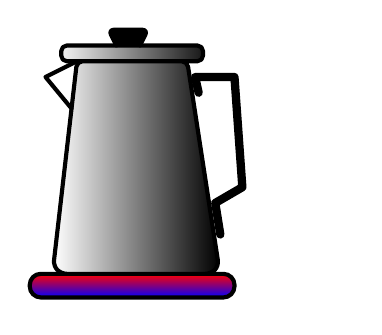
\begin{tikzpicture}[scale = 1, line join=round, line cap=round, >=stealth,line width=1.
					5]
					\draw[rounded corners=4,top color=red,bottom color=blue] (0,0) rectangle (2.6,0.3);
					\draw[rounded corners=2,left color=white,right color=black] (0.6,3)--(0.3,0.4)
					--(0.4,0.3) -- (2.3,0.3) --(2.4,0.4)--(2,3)--cycle (0.4,3) rectangle (2.2,3.2);
					\draw[rounded corners=2,fill=black] (1.1,3.2)--(1,3.4) -- (1.5,3.4)--(1.4,3.2);
					\draw[line width=3] (2.145,2.6)-- (2.1,2.8) -- (2.6,2.8) -- (2.7,1.4) -- (2.356,1.2)
					--(2.42,0.8);
					\draw (0.6,3) -- (0.2,2.8)--(0.53,2.4);
					\draw (4,0) node {};
			\end{tikzpicture}} & Điện áp & \multicolumn{1}{|l|}{220 V – 50 Hz} \\
			\cline{2-3}
			& \multirow{2}[0]{*}{Công suất} & \multicolumn{1}{|l|}{2500 W khi nước chưa sôi} \\
			& & \multicolumn{1}{|l|}{1700 W khi nước sôi} \\
			\cline{2-3}
			& \multirow{2}[0]{*}{Chế độ an toàn} & \multicolumn{1}{|l|}{Tự hạ công suất khi nước sôi } \\
			& & \multicolumn{1}{|l|}{và tự ngắt khi cạn nước} \\
			\cline{2-3}
			& \multirow{2}[0]{*}{Chất liệu} & \multicolumn{1}{|l|}{Vỏ ấm bằng thuỷ tinh có khả năng} \\
			& & \multicolumn{1}{|l|}{ cách nhiệt tốt, đế ấm bằng inox 304} \\
			\cline{2-3}
			& \multicolumn{2}{|c|}{\textit{Thông số kĩ thuật của ấm điện}} \\
			\cline{2-3} 
		\end{tabular}
	\end{center} 
	Ngoài ra, học sinh còn dùng cân điện tử để cân lượng nước còn lại trong ấm và dùng đồng hồ để đo thời gian đun. Khi nước sôi ở $100^\circ C$ thì học sinh mở nắp ấm cho hơi nước dễ bay ra và bắt đầu ghi lại số liệu khi lượng nước còn lại trong ấm là $350\ g$. Đồ thị sự phụ thuộc của khối lượng nước $m$ còn lại trong ấm vào thời gian đun như đồ thị bên dưới.
	\begin{center}
		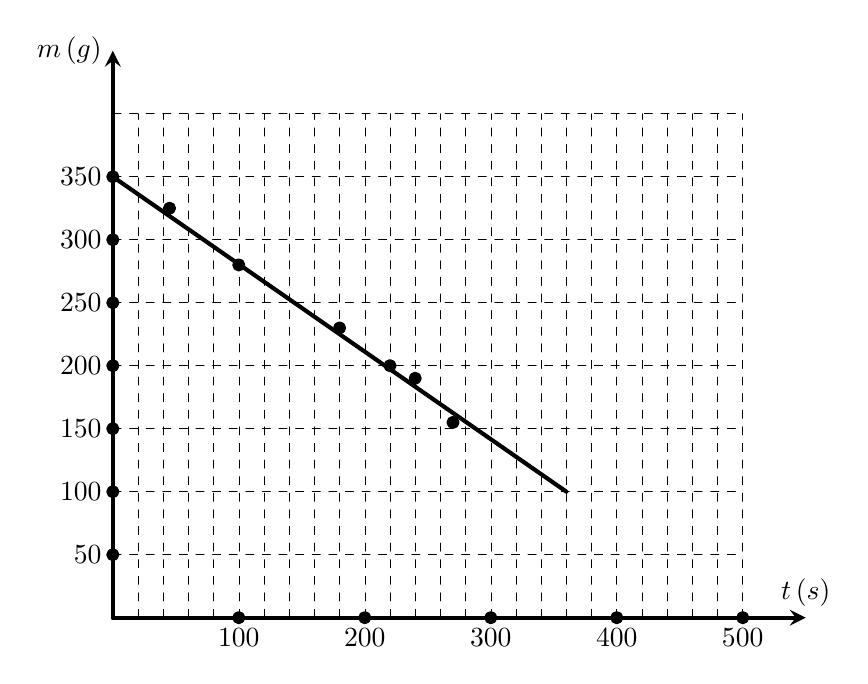
\begin{tikzpicture}[scale = 0.8, line join=round, line cap=round, >=stealth,line
			width=1.5]
			\draw[dashed,line width=0.2] (0,0) grid[xstep=0.4,ystep=1] (10,8);
			\draw[->] (0,0)--(11,0) node [above] {$t\left(s\right)$};
			\draw[->] (0,0)--(0,9) node [left] {$m\left(g\right)$};
			\foreach \x/\y in {0.9/6.5,2/5.6,3.6/4.6,4.4/4,4.8/3.8,5.4/3.1}
			{\draw [fill=black] (\x,\y) circle (2pt);}
			\foreach \x in {100,200,300,400,500} {\draw[fill=black] ({2*\x/100},0) circle (2pt) node [below] {\x};}
			\foreach \x in {50,100,...,350} {\draw[fill=black] (0,{\x/50}) circle (2pt) node [left] {\x};}
			\draw (0,7) -- (7.2,2);
		\end{tikzpicture}
	\end{center}
	
	Biết rằng khi nước chưa sôi thì hiệu suất đun nước của ấm bằng $96\%$ còn khi nước sôi thì hiệu suất ấm đun giảm xuống còn $92\%$, nhiệt dung riêng của nước là $4200\ J/kg.K$.
	\choiceTF[t]
	{\True Nếu khi nước sôi không mở nắp ấm thì thời gian để đun cạn nước trong ấm sẽ tăng lên}
	{Độ hụt khối lượng của nước trong ấm sau mỗi giây bằng $0,34\ g/s$}
	{Nhiệt hoá hơi riêng của nước trong thí nghiệm này bằng $2,33\ MJ/kg$}
	{Tổng thời gian đun nước đến khi cạn bằng $556,39\ s$}
	\loigiai{
		Nếu khi nước sôi không mở nắp ấm thì thời gian để đun cạn nước trong ấm sẽ tăng lên do đậy nắp ấm làm cho hơi nước thoát ra ngoài khó hơn nên việc hoá hơi gặp khó khăn hơn.\\
		\iconX Độ hụt khối lượng của nước trong ấm sau mỗi giây bằng: $\dfrac{\Delta m}{\Delta \tau }=\dfrac{350-200}{220}=0,68\,g/s$.\\
		\iconX Năng lượng ấm toả ra: $A=P.\left(\tau_2-\tau_1\right)$\\
		Năng lượng nước thu vào trong quá trình bay hơi: $Q=\left(m_1-m_2\right).L$\\
		Do hiệu suất trong quá trình sôi là $92\%$ nên ta có:
		$Q=92\%A\Rightarrow \left( m_1-m_2 \right)L=0,92.P.\left(\tau_2-\tau_1\right)$\\
		$\Rightarrow \left(0,35-0,2\right).L=0,92.1700.\left(220-0\right) \Rightarrow L= 2,29.10^6\ J/kg$.\\ 
		\iconX Nhiệt lượng $380\ g$ nước thu vào để bay hơi hoàn toàn $380\ g$ ở nhiệt độ sôi là:\\ 
		$Q_2=m.L=0,38.2,29.10^6=870200\ J$.\\
		Thời gian bếp đun từ lúc sôi đến khi bay hơi hết:\\ $t_2=\dfrac{A_2}{P_2}=\dfrac{\dfrac{Q_2}{H_2}}{P_2}=\dfrac{\dfrac{870200}{0,92}}{1700}=556,39\ s$\\
		Nhiệt lượng $380\ g$ nước thu vào để tăng đến nhiệt độ sôi:\\ 
		$Q_1=mc\Delta T=0,38.4200.\left(100-20\right)=127680\ J$.\\
		Thời gian bếp đun từ lúc sôi đến khi bay hơi hết:\\ $t_1=\dfrac{A_1}{P_1}=\dfrac{\dfrac{Q_1}{H_1}}{P_1}=\dfrac{\dfrac{127680}{0,96}}{2500}=53,20\ s$.\\
		Tổng thời gian đun nước: $t=t_1+t_2=609,59\ s$.
	} 
\end{ex}
\begin{ex}%group
	\immini[thm]{Một vật đơn chất từ trạng thái rắn, được cung cấp nhiệt với công suất không đổi. Đồ thị (hình bên) thể hiện sự thay đổi nhiệt độ $t\left({ }^\circ C\right)$ của khối chất theo thời gian $\tau$ (phút). Bỏ qua sự trao đổi nhiệt với môi trường.}{\begin{tikzpicture}[scale = 0.8, line join=round, line cap=round, >=stealth,line width=1.5]
			\draw[->] (0,-2.5)--(0,4.5) node[right] {$\tau\ \left(^{\circ}C\right)$};
			\draw[->] (0,0)--(6.5,0) node[right] {$t\ \left(\text{phút}\right)$};
			\draw[dashed,line width=0.5,ystep=1,xstep=0.2] (0,-2) grid (6,4);
			\foreach \x in {5,10,...,30} {\draw[fill=black] ({\x/5},0) circle (2pt) node [above] {\x};}
			\draw[fill=black] (0,-2) circle (2pt) node [left] {$-20$};
			\draw[fill=black] (0,0) circle (2pt) node [left] {$0$};
			\draw[fill=black] (0,2) circle (2pt)  node [left] {$20$};
			\draw (0,-2) -- (0.2,-1) -- (2.6,-1) -- (4.8,3) -- (5.6,3);
	\end{tikzpicture}}
	\choiceTFt
	{Nhiệt độ sôi của chất bằng $-10^\circ C$}
	{\True Thời gian khối chất nóng chảy là $12$ phút}
	{Gọi nhiệt dung riêng của chất ở thể rắn, lỏng lần lượt là ${c}_{{r}}$ và ${c}_{\ell}$, thì ${c}_{\ell}=11 {c}_{{r}}$}
	{\True Chênh lệch giữa nhiệt độ nóng chảy và nhiệt độ sôi bằng $40\ K$}
	\loigiai{	\begin{itemchoice}
			\itemch Nhiệt độ nóng chảy của chất bằng $-10^\circ C$
			\itemch Thời gian khối chất nóng chảy là $13-1=12$ phút
			\itemch $P \Delta \tau=m c \Delta t \Rightarrow \dfrac{\Delta \tau_{l}}{\Delta \tau_{r}}=\dfrac{c_{l} \Delta t_{l}}{c_{r} \Delta t_{r}} \Rightarrow \dfrac{24-13}{1}=\dfrac{c_{l} . 40}{c_{r} . 10} \Rightarrow \dfrac{c_{l}}{c_{r}}=2,75$ 
			\itemch $\Delta T_{l}=\Delta t_{l}=40(K)$
		\end{itemchoice}
	}
\end{ex}
\subsubsection*{PHẦN 3. Thí sinh trả lời từ câu 1 đến câu 6.}
\setcounter{ex}{0}
\begin{ex}%group
	Một học sinh làm thí nghiệm đo nhiệt hóa hơi riêng của nước (cân điện tử, ấm siêu tốc, đồng hồ đo thời gian, chai nước). Biết ấm đun có công suất trung bình là $\mathcal{P}=1500\ W$. Khi nước bắt đầu sôi, khối lượng nước trong ấm đo được bằng cân điện tử là $m_0=300\ g$, lúc này học sinh mở nắp ấm để nước bay hơi, sau khoảng thời gian $77$ giây thì thấy số chỉ trên cân điện tử còn $m=250\ g$. Bỏ qua sự trao đổi nhiệt với môi trường bên ngoài. Nhiệt hóa hơi riêng của nước bằng $x.10^{4}\ J/kg$. Tìm x.
	\shortans[oly]{$231$}
	\loigiai{\begin{itemize}
			\item Ta có: Ta có: $Q=m.L=P.t\Rightarrow 0,05.L=1500.77\Rightarrow L=231.10^4(J/kg)$.
	\end{itemize}}
\end{ex}
\begin{ex}%group
	Trong một bình thành mỏng thẳng đứng diện tích đáy $S=100\ cm^2$ chứa nước và nước đá ở nhiệt độ $t_1=0^\circ C$, khối lượng nước gấp $10$ lần khối lượng nước đá. Một thiết bị bằng thép được đốt nóng tới $t_2=80^\circ C$ rồi nhúng ngập trong nước, ngay sau đó mức nước trung bình dâng lên cao thêm $h=3\ cm$. Biết rằng khi trạng thái cân bằng nhiệt được thiết lập trong bình nhiệt độ của nó là $t=5^\circ C$. Bỏ qua sự trao đổi nhiệt với bình và môi trường. Cho biết nhiệt dung riêng của nước là $4200\ J/kg.K$, của thép là $500\ J/kg.K$. Nhiệt nóng chảy riêng của nước đá là $330\ kJ/kg$, khối lượng riêng của thép là $7700\ kg/m^3$. Khối lượng của nước lúc đầu trong bình bằng bao nhiêu kg (làm tròn kết quả đến chữ số hàng phần trăm)?
	\shortans[oly]{$1,54$}
	\loigiai{
		\begin{itemize}
			\item Gọi khối lượng nước trong bình là $m(kg)$. Suy ra khối lượng nước đá trong bình là $\dfrac{m}{10}(kg)$.
			\item Thể tích khối thép là: $V=S.h=100.3=300(cm^3)=300.10^{-6}(m^3)$
			\item Khối lượng của khối thép là: $m_1=D.V=7700.300.10^{-6}=2,31(kg)$
			\item Nhiệt lượng cho khối thép tỏa ra là: $Q_1=m_1c_1\Delta t=2,31.500.(80-5)=86625(J)$.
			\item Nhiệt lượng nước và nước đá thu vào:
			$$Q_2=\dfrac{m}{10}.\lambda \left(\dfrac{m}{10}+m\right).c_2\Delta t=\dfrac{m}{10}.330.10^3+ \left( \dfrac{m}{10}+m\right).4200.(5-0)$$
			\item Phương trình cân bằng nhiệt, ta có:
			$$Q_1=Q_2\Rightarrow 86625=\dfrac{m}{10}.330.10^3+ \left( \dfrac{m}{10}+m\right).4200.(5-0)\Rightarrow m\approx1,54(kg)$$
		\end{itemize}
		
	}
\end{ex}


\textit{Sử dụng các thông tin sau cho Câu 3 và Câu 4:} Vào mùa hè, một số người thường có thói quen uống trà đá. Để có một cốc trà đá, người chủ quán rót khoảng $0,05\ kg$ nước trà nóng ở $80^\circ C$ vào cốc, sau đó cho tiếp $m\ (g)$ đá viên ở $0^\circ C$. Cuối cùng được cốc trà đá ở nhiệt độ phù hợp nhất là $10^\circ C$. Biết nhiệt dung riêng của nước là $4,2\ kJ/kg.K$; nhiệt nóng chảy riêng của nước đá là ${3,33.10}^{5}\ J/kg$.

%---------------------Câu 3
\begin{ex}
	Nhiệt lượng do nước trà tỏa ra để hạ nhiệt độ từ  $80^\circ C$ xuống  $10^\circ C$ là bao nhiêu $kJ$ (làm tròn kết quả đến chữ số hàng phần mười)?
	\shortans[oly]{$14,7$}%Thay đáp án chuẩn 
	\loigiai{Nhiệt lượng do nước trà tỏa ra để hạ nhiệt độ từ $80^\circ C$ xuống $10^\circ C$ là\\
		$Q_1 = m_nc_n\Delta t = 0,05.4200.(80-10)=14700\ (J)=14,7\ kJ$}
\end{ex}

%---------------------Câu 4
\begin{ex}
	Hao phí do tỏa nhiệt ra môi trường là 10\%. Giá trị của m là bao nhiêu gam (làm tròn kết quả đến chữ số hàng phần mười)?
	\shortans[oly]{$35,3$}%Thay đáp án chuẩn 
	\loigiai{Nhiệt lượng do nước đá thu vào là: \\ 
		$Q_2=m.\lambda + mc\Delta t=m.3,33.10^5+m.4200.(10-0)=3,75.10^5.m\ (J)$\\
		Do hao phí tỏa nhiệt ra môi trường là $10\%$ nên theo phương trình cân bằng nhiệt, ta có:\\
		$90\%Q_1=Q_2\Rightarrow 90\%.14700=3,75.10^5m \Rightarrow m = 0,03528\ (kg) \approx 35,3\ (g)$}
\end{ex}
\begin{ex}%group%group
	Trong một bình lớn cách nhiệt đã được hút hết khí và hơi nước. Lúc đầu có hỗn hợp nước và nước đá có khối lượng tổng cộng $m$ và nhiệt độ $0^\circ C$. Do nước lỏng bay hơi và phần còn lại của nước bị đông đặc nên ở cuối quá trình này trong bình có lượng nước đá tổng cộng là $0,92\ m$. Cho biết nhiệt nóng chảy riêng của nước đá và nhiệt hóa hơi riêng của nước có giá trị lần lượt là $\lambda = 3,3.10^5\ J/kg$; $L = 2,3.10^6\ J/kg$. Tính tỉ số khối lượng nước đá so với khối lượng nước lúc đầu (làm tròn kết quả đến chữ số hàng phần trăm)?
\shortans[oly]{0,57}
	\loigiai{
		\begin{itemize}
			\item Gọi khối lượng nước và nước đá ban đầu là $m_n$ và $m_d$, ta có: $m_n + m_d = m (1).$
			\item Một phần nước $m'$ đông đặc và phần $(m_n - m' )$ bay hơi, theo phương trình cân bằng nhiệt, ta có:
			$m'\lambda = (m_n - m')L \Rightarrow m' = \dfrac{L}{\lambda +L}m_n = \dfrac{2,3.10^6}{3,3.10^5 + 2,3.10^6}m_n = \dfrac{230}{263}m_n$.
			\item Ở cuối quá trình, ta có: $m' + m_d = 0,92m \Rightarrow\dfrac{230}{263}m_n + m_d = 0,92m$ \\
			Từ (1) và (2)$\Rightarrow$ $\begin{cases}
				m_n = \dfrac{526}{825}m \\
				m_d = \dfrac{299}{825}m 
				
			\end{cases}$
			$\Rightarrow \dfrac{m_d}{m_n} = \dfrac{299}{526} \approx 0,57$.
		\end{itemize}
		
	}
	
\end{ex}

\begin{ex}%group
	\immini[thm]{Dùng ấm điện có công suất định mức $500\ W$ để đun sôi nồi nước chè có khối lượng tổng cộng $2,5\ kg$ (không kể khối lượng của ấm). Biết nhiệt dung riêng của hỗn hợp nước chè trong ấm phụ thuộc nhiệt độ như đồ thị hình bên. Nhiệt độ ban đầu của nước là $24^\circ C$; coi nhiệt độ sôi của nước chè là $100^\circ C$. Nhiệt lượng để đun sôi nước chè chiếm $80\%$ nhiệt lượng mà dây may so trong ấm tỏa ra. Biết ấm điện hoạt động bình thường. Thời gian để đun sôi nước chè là bao nhiêu phút (làm tròn kết quả đến chữ số hàng phần mười)?}
	{\begin{tikzpicture}[scale = 1, line join=round, line cap=round, >=stealth]
			\path
			(0,0)coordinate(O)
			(5,0)coordinate(x)
			(0,4)coordinate(y)
			;
			\draw [->](O)--(x);
			\draw [->](O)--(y);
			\node at (5,0.5) {$t\ (^\circ C)$};
			\node at (0,4.5) {$c\ (J/kg.K)$};
			\draw[dashed] (0,1.5) -- (4,1.5) -- (4,0);
			\draw[dashed] (1,0) -- (1,3) -- (0,3);
			\draw[line width=1.2pt,blue] (1,3) -- (4,1.5);
			\node[left] at (0,1.5) {$3680$};
			\node [left]at (0,3) {$4200$};
			\node[below] at (1,0) {$24$};
			\node[below]  at (4,0) {$100$};
	\end{tikzpicture}}
	\par \shortans[oly]{31,2}
	\loigiai{
		\begin{itemize}
			\item Nhiệt dung riêng trung bình của nước chè trong khoảng nhiệt độ từ $24^\circ C$ đến $100^\circ C$ là:\\
			$c=\dfrac{4200+3680}{2}=3940 \ J/kg.K$
			\item Ta có: $Q=m.c.\Delta t=P.t.80\%\Rightarrow 2,5.3940.(100-24)=500.t.80\%\Rightarrow t=1871.5 \ s\approx 31,2$ phút 
			
		\end{itemize}
	}
\end{ex}
